\section{Primeiro Experimento - Interferência Via Cache}

O primeiro experimento tem como objetivo avaliar o comportamento e a capacidade de isolamento do hipervisor sob condições de contenção
de recursos. Para isso, utilizam-se duas instâncias de \glspl{vm} executando o \gls{so} EPOS, configuradas com perfis de carga distintos
e concorrentes. As tarefas foram programadas para execução periódica, permitindo observar a eficácia do hipervisor no gerenciamento
e na alternância entre fluxos de trabalho com diferentes intensidades e frequências.

\begin{itemize}
    \item \gls{vm} 1 - EPOS com alta demanda de CPU: Esta instância simula uma carga intensiva de processamento por meio da execução de
		uma versão iterativa do cálculo da sequência de Fibonacci, conforme detalhado no Algoritmo~\ref{alg:fibonacci_cpu_hungry}.
		A \gls{vm} é configurada para disparar esse algoritmo periodicamente a cada 5.000~\si{\micro\second}.
\end{itemize}

\begin{algorithm}[H]
\caption{Fibonacci Iterativo}
\label{alg:fibonacci_cpu_hungry}
\begin{algorithmic}[1]
\Procedure{Fibonacci}{$number \gets 100000$}
    \State $a \gets 0$
    \State $b \gets 1$
    \State $fib \gets 0$
    \For{$i \gets 0$ \textbf{to} $number - 1$}
        \State $fib \gets a + b$
        \State $a \gets b$
        \State $b \gets fib$
    \EndFor
\EndProcedure
\end{algorithmic}
\end{algorithm}

\begin{itemize}
    \item \gls{vm} 2 - EPOS com alta demanda de memória: Esta instância estressa o subsistema de memória por meio da aplicação iterativa
		de uma operação de convolução bidimensional sobre uma imagem sintética de $512 \times 512$ pixels, utilizando um kernel de
		tamanho $3 \times 3$. A implementação deste fluxo de trabalho está descrita no Algoritmo~\ref{alg:convolution_memory_hungry}.
		Essa \gls{vm} executa a tarefa periodicamente a cada 100.000~\si{\micro\second}.
\end{itemize}

\begin{algorithm}[H]
\caption{Convolução Bidimensional}
\label{alg:convolution_memory_hungry}
\begin{algorithmic}[1]
\Procedure{Convolution}{}
    \State Matrix $A[512][512]$
    \State Matrix $C[512][512]$
    \State Kernel $K[3][3]$

    \For{$Iteration \gets 1$ \textbf{to} $5$}
        \For{$i \gets 1$ \textbf{to} $510$}
            \For{$j \gets 1$ \textbf{to} $510$}
                \State $sum \gets 0$
                \For{$x \gets -1$ \textbf{to} $1$}
                    \For{$y \gets -1$ \textbf{to} $1$}
                        \State $sum \gets sum + A[i+x][j+y] \times K[x+1][y+1]$
                    \EndFor
                \EndFor
                \State $C[i][j] \gets sum$
            \EndFor
        \EndFor
    \EndFor
\EndProcedure
\end{algorithmic}
\end{algorithm}

Os tempos de execução de cada iteração das aplicações executadas nas \glspl{vm} ao longo de um intervalo de cinco minutos são
apresentados nas Figuras \ref{fig:16_without_linux}, \ref{fig:23_without_linux}, \ref{fig:16_with_linux}, \ref{fig:23_with_linux},
\ref{fig:16_with_linux_bandwidth} e \ref{fig:23_with_linux_bandwidth}. Cada gráfico mostra a evolução temporal do tempo de execução
das tarefas do EPOS sob diferentes cenários de compartilhamento de recursos entre máquinas virtuais.

As Figuras \ref{fig:16_without_linux} e \ref{fig:23_without_linux} apresentam os resultados obtidos quando apenas a \gls{vm}
contendo o EPOS está ativa. Nessa configuração observa-se um comportamento relativamente estável, com pequenas oscilações atribuídas
ao escalonamento normal do hipervisor. Os tempos de execução das cargas baseadas em CPU e memória permanecem próximos aos valores de
referência, caracterizando o desempenho esperado na ausência de interferência externa.

Nas Figuras \ref{fig:16_with_linux} e \ref{fig:23_with_linux} é introduzida uma segunda \gls{vm} executando um Linux sem
carga computacional. Embora exista compartilhamento dos núcleos físicos entre as máquinas virtuais, o impacto observado sobre os
tempos de execução do EPOS é reduzido. As variações permanecem próximas às observadas no cenário de referência.

Por fim, as Figuras \ref{fig:16_with_linux_bandwidth} e \ref{fig:23_with_linux_bandwidth} mostram o comportamento do sistema quando a
\gls{vm} com Linux executa uma carga intensiva de memória, projetada para gerar elevado tráfego no subsistema de memória e frequentes
invalidações das linhas de cache compartilhadas entre os núcleos. Nesse cenário, observa-se um aumento expressivo nos tempos de
execução da aplicação do EPOS com carga baseada em memória. O efeito torna-se evidente a partir do momento em que a carga
concorrente é iniciada, indicando uma degradação diretamente associada à contenção dos recursos de memória e à redução da
efetividade do cache.

Em contrapartida, as aplicações com carga predominantemente computacional apresentam apenas pequenas variações em seus tempos de
execução, mesmo diante da atividade intensiva de memória da \gls{vm} Linux. Esse comportamento sugere a existência de um
mecanismo significativo de interferência entre as máquinas virtuais associado ao compartilhamento da hierarquia de cache.
Nesse contexto, como a quantidade de memória alocada para cada \gls{vm} é elevada, estratégias convencionais de particionamento
de memória tendem a ser insuficientes para mitigar esse efeito. Assim, soluções efetivas dependem diretamente da capacidade de
isolamento provida por controladores específicos de cache — por exemplo, mecanismos de particionamento ou alocação de vias — ou,
em cenários experimentais mais extremos, da desativação completa dos níveis de cache compartilhados, de modo a eliminar a
fonte de interferência observada.

\begin{figure}[ht]
    \centering
    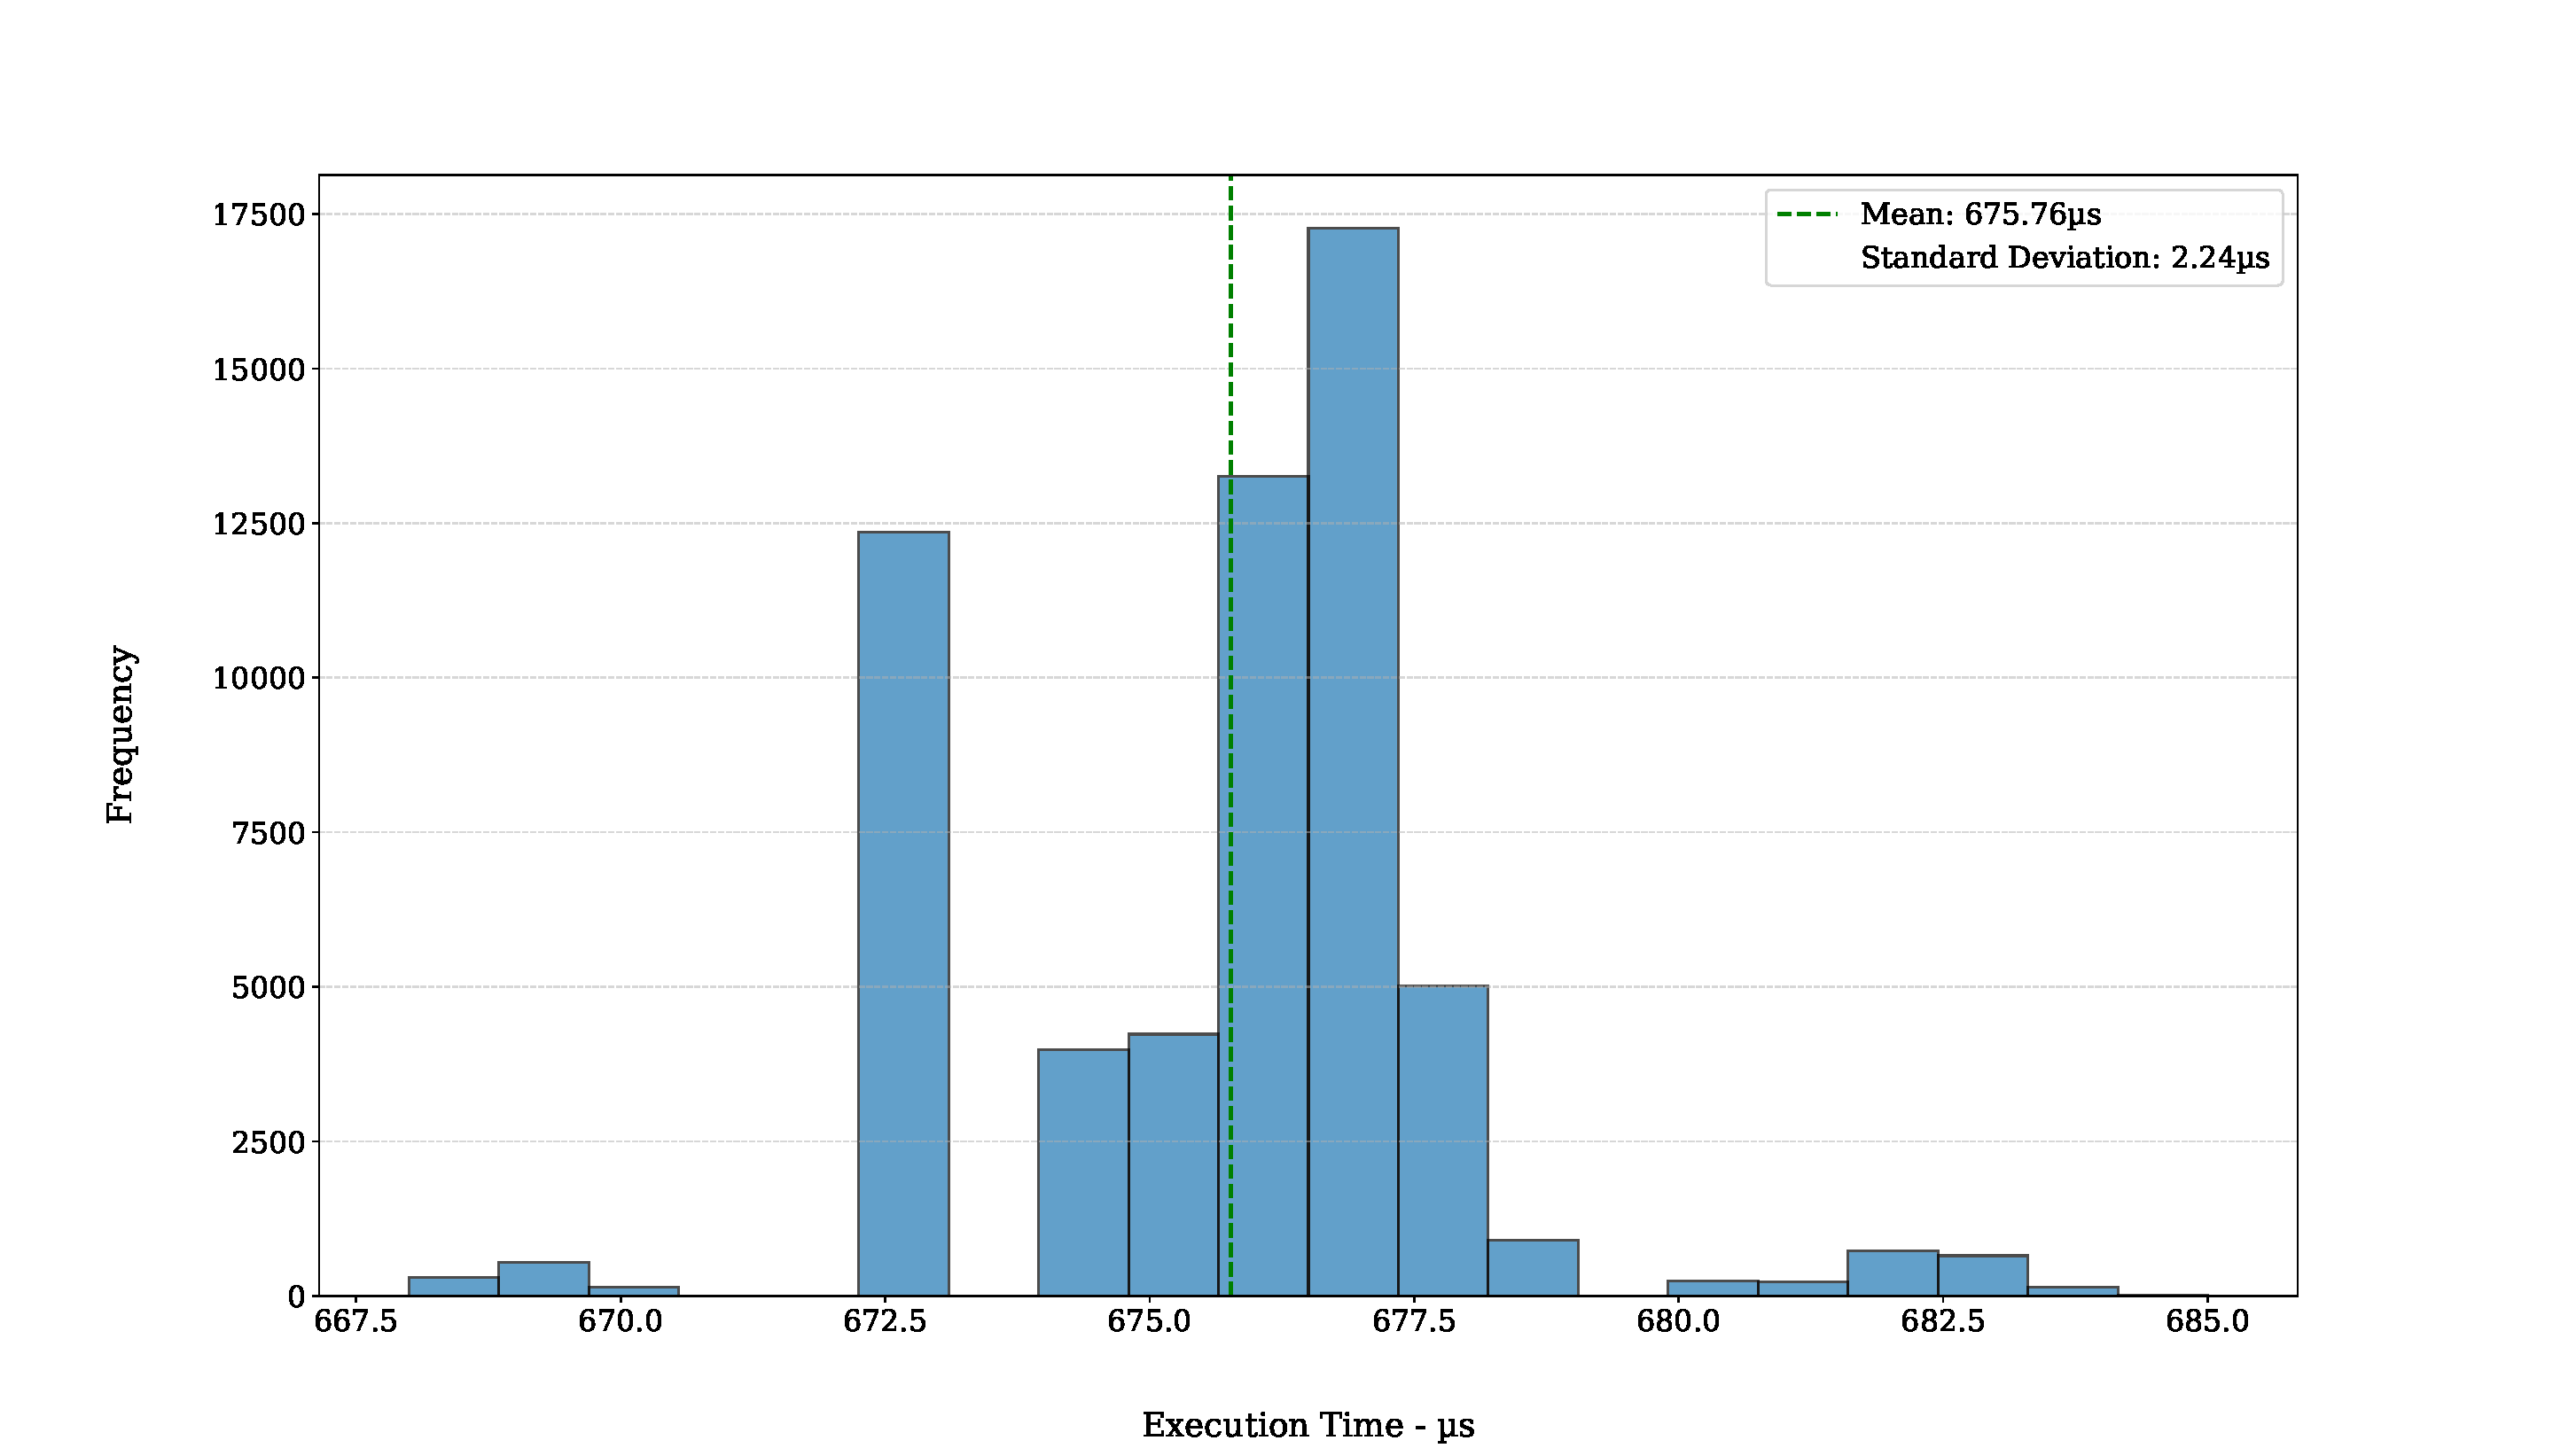
\includegraphics[width=0.95\textwidth]{images/16_without_linux.pdf}
	\caption{Tempos de Execução Das Iterações de Uma \gls{vm} Com Carga em CPU - Sem Linux.}
    \label{fig:16_without_linux}
\end{figure}

\begin{figure}[ht]
    \centering
    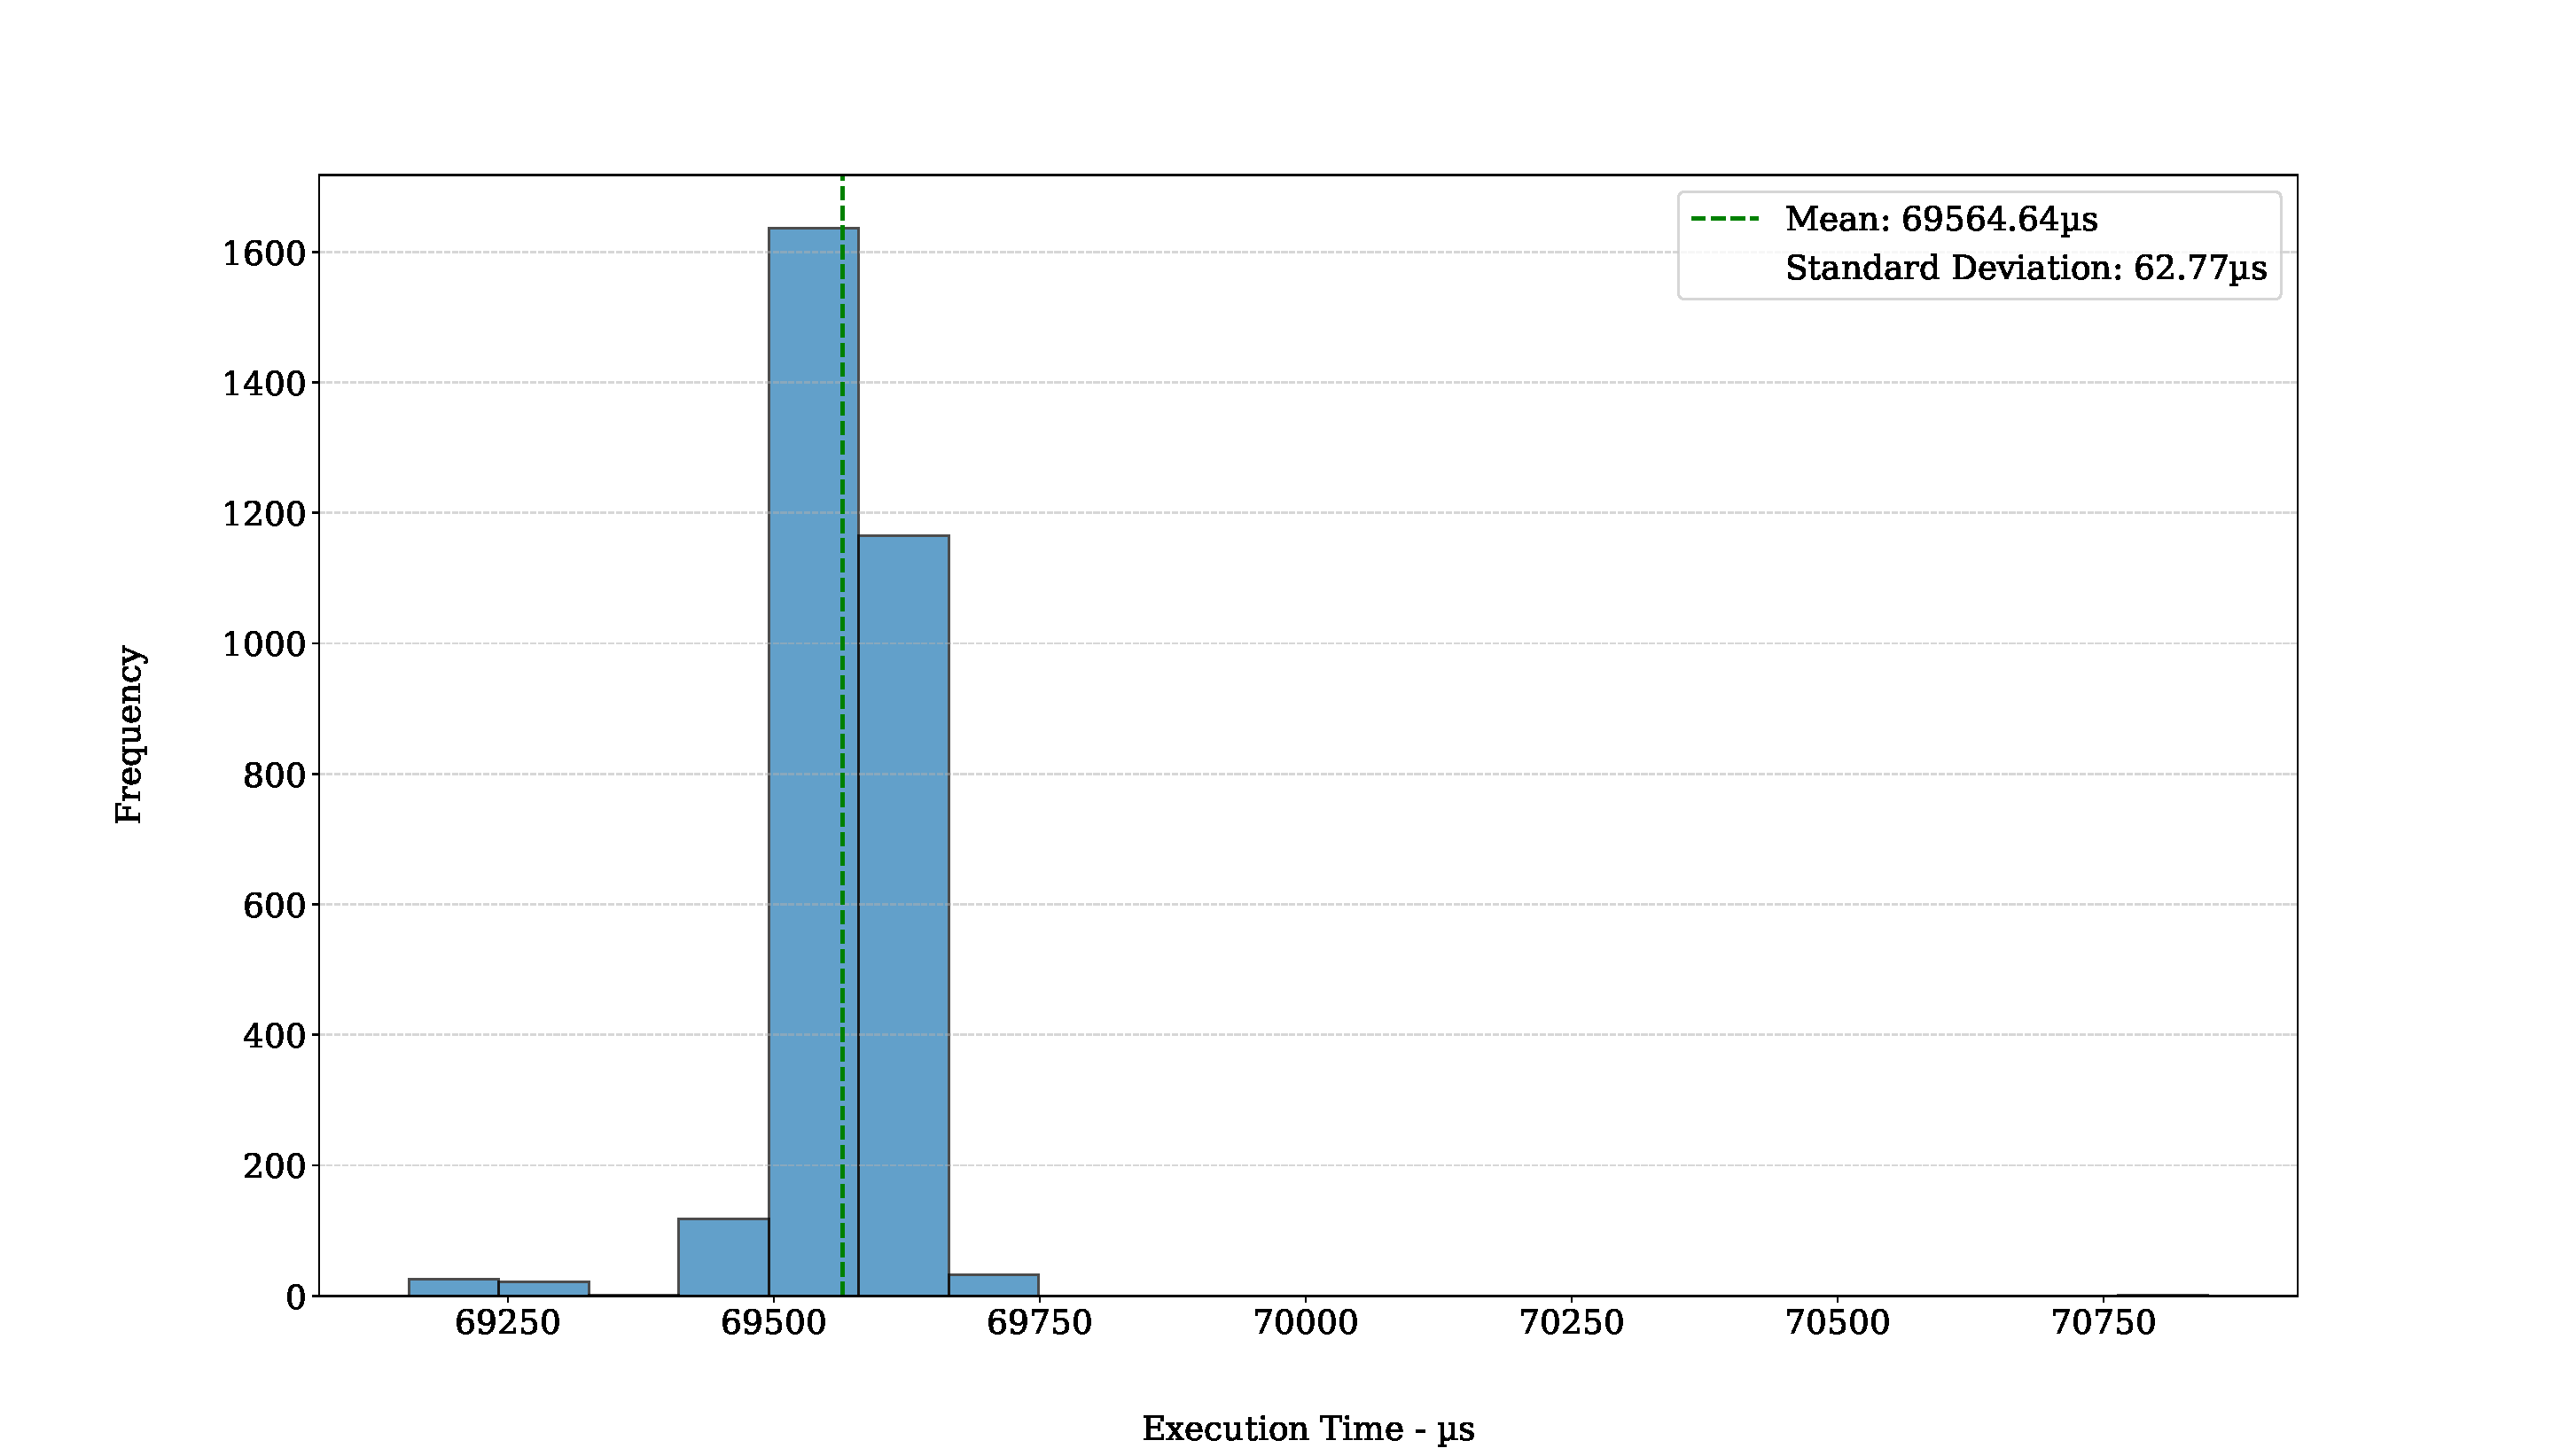
\includegraphics[width=0.95\textwidth]{images/23_without_linux.pdf}
	\caption{Tempos de Execução Das Iterações de Uma \gls{vm} Com Carga em Memória - Sem Linux.}
    \label{fig:23_without_linux}
\end{figure}

\begin{figure}[ht]
    \centering
    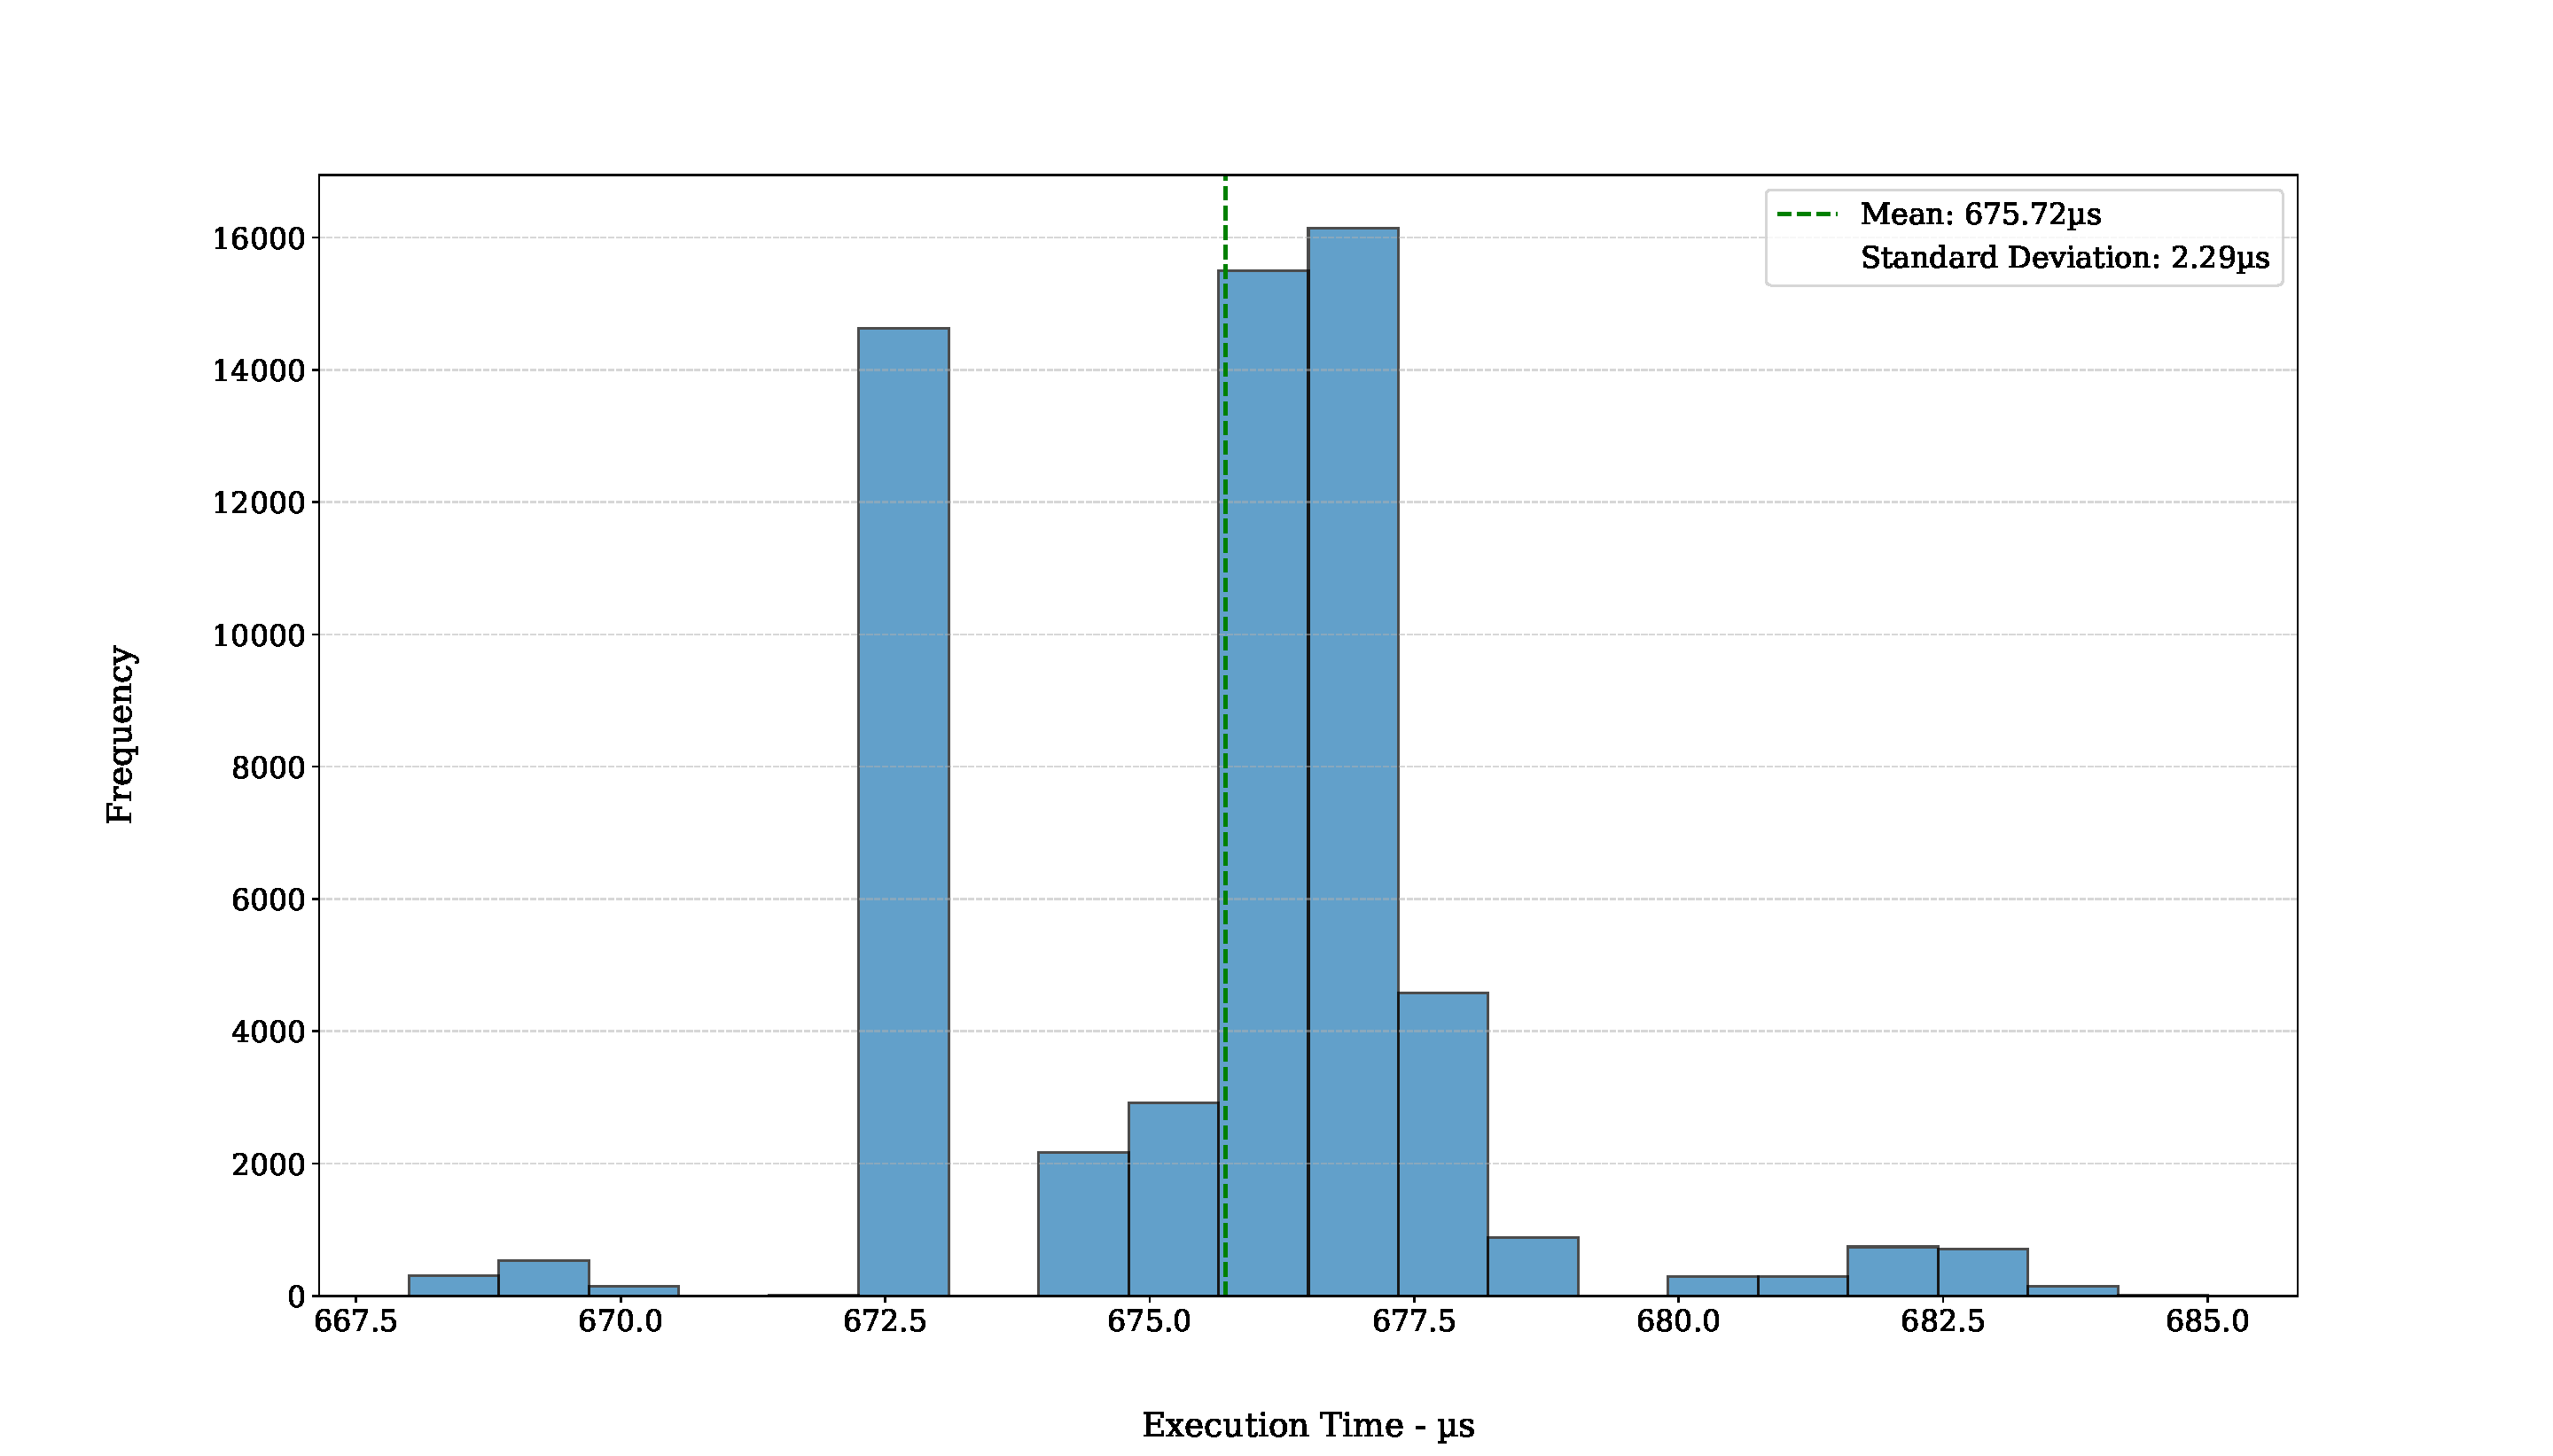
\includegraphics[width=0.95\textwidth]{images/16_with_linux.pdf}
	\caption{Tempos de Execução Das Iterações de Uma \gls{vm} Com Carga em CPU - Com Linux.}
    \label{fig:16_with_linux}
\end{figure}

\begin{figure}[ht]
    \centering
    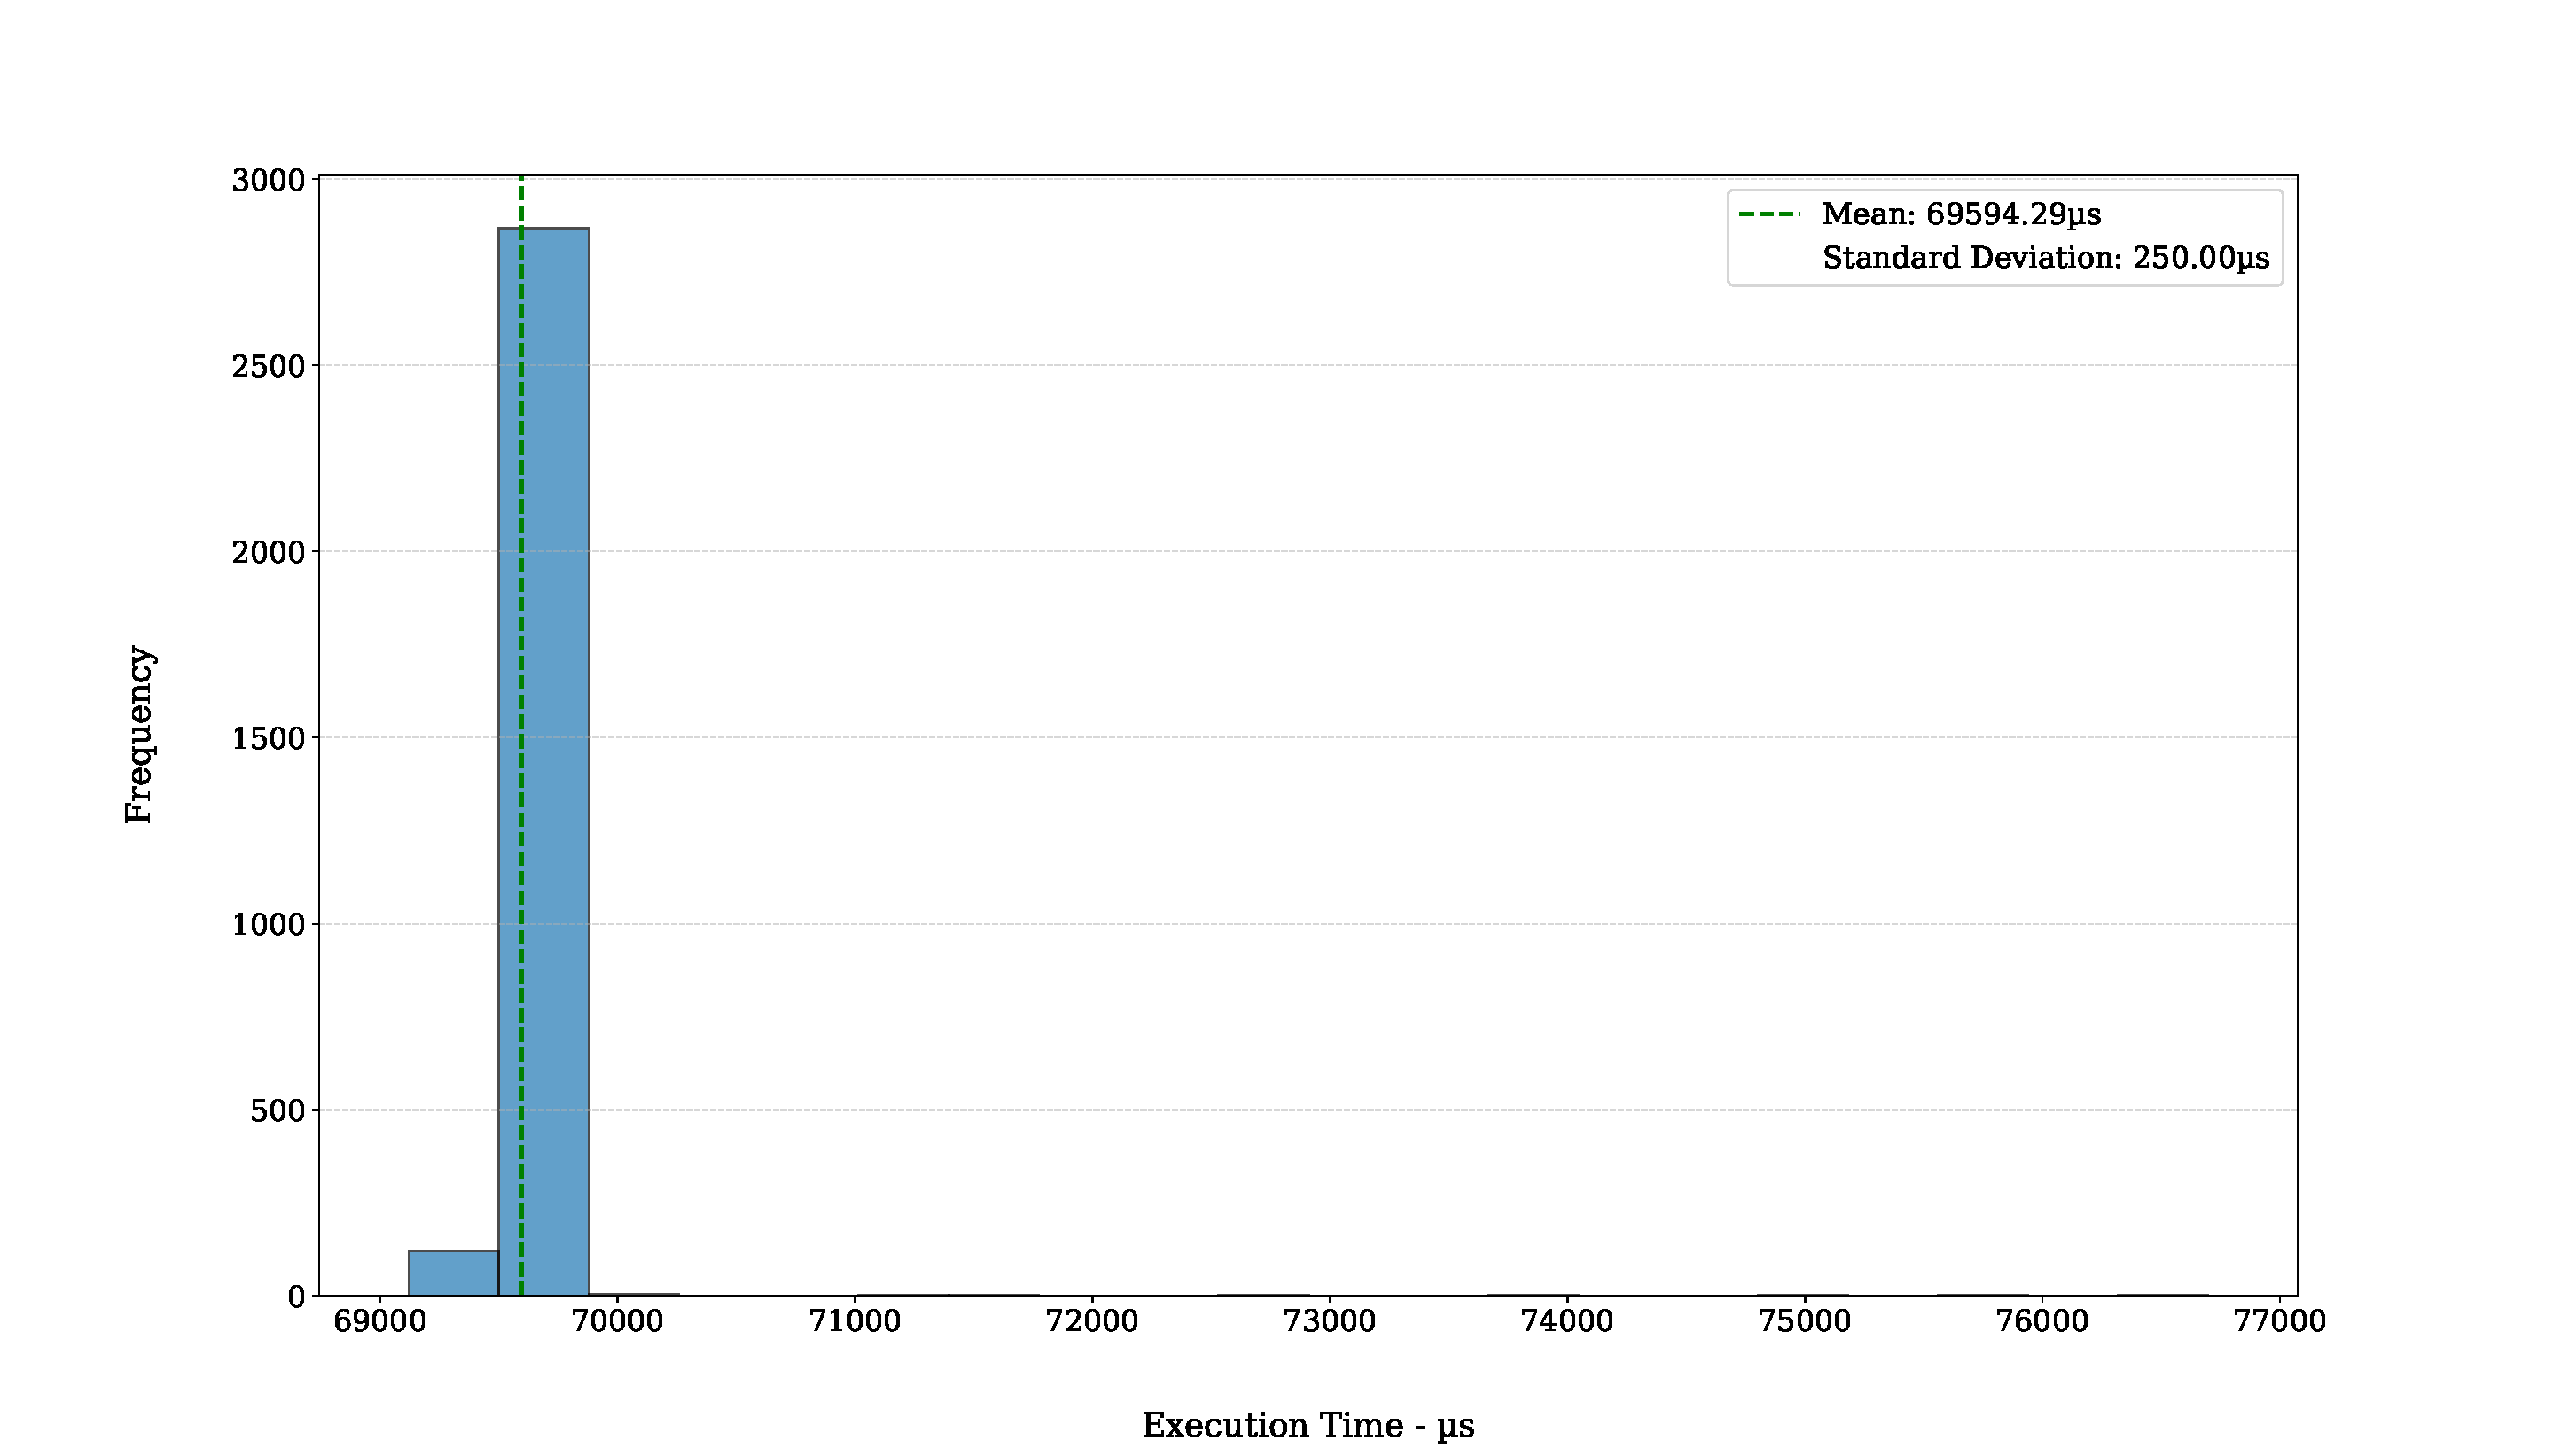
\includegraphics[width=0.95\textwidth]{images/23_with_linux.pdf}
	\caption{Tempos de Execução Das Iterações de Uma \gls{vm} Com Carga em Memória - Com Linux.}
    \label{fig:23_with_linux}
\end{figure}


\begin{figure}[ht]
    \centering
    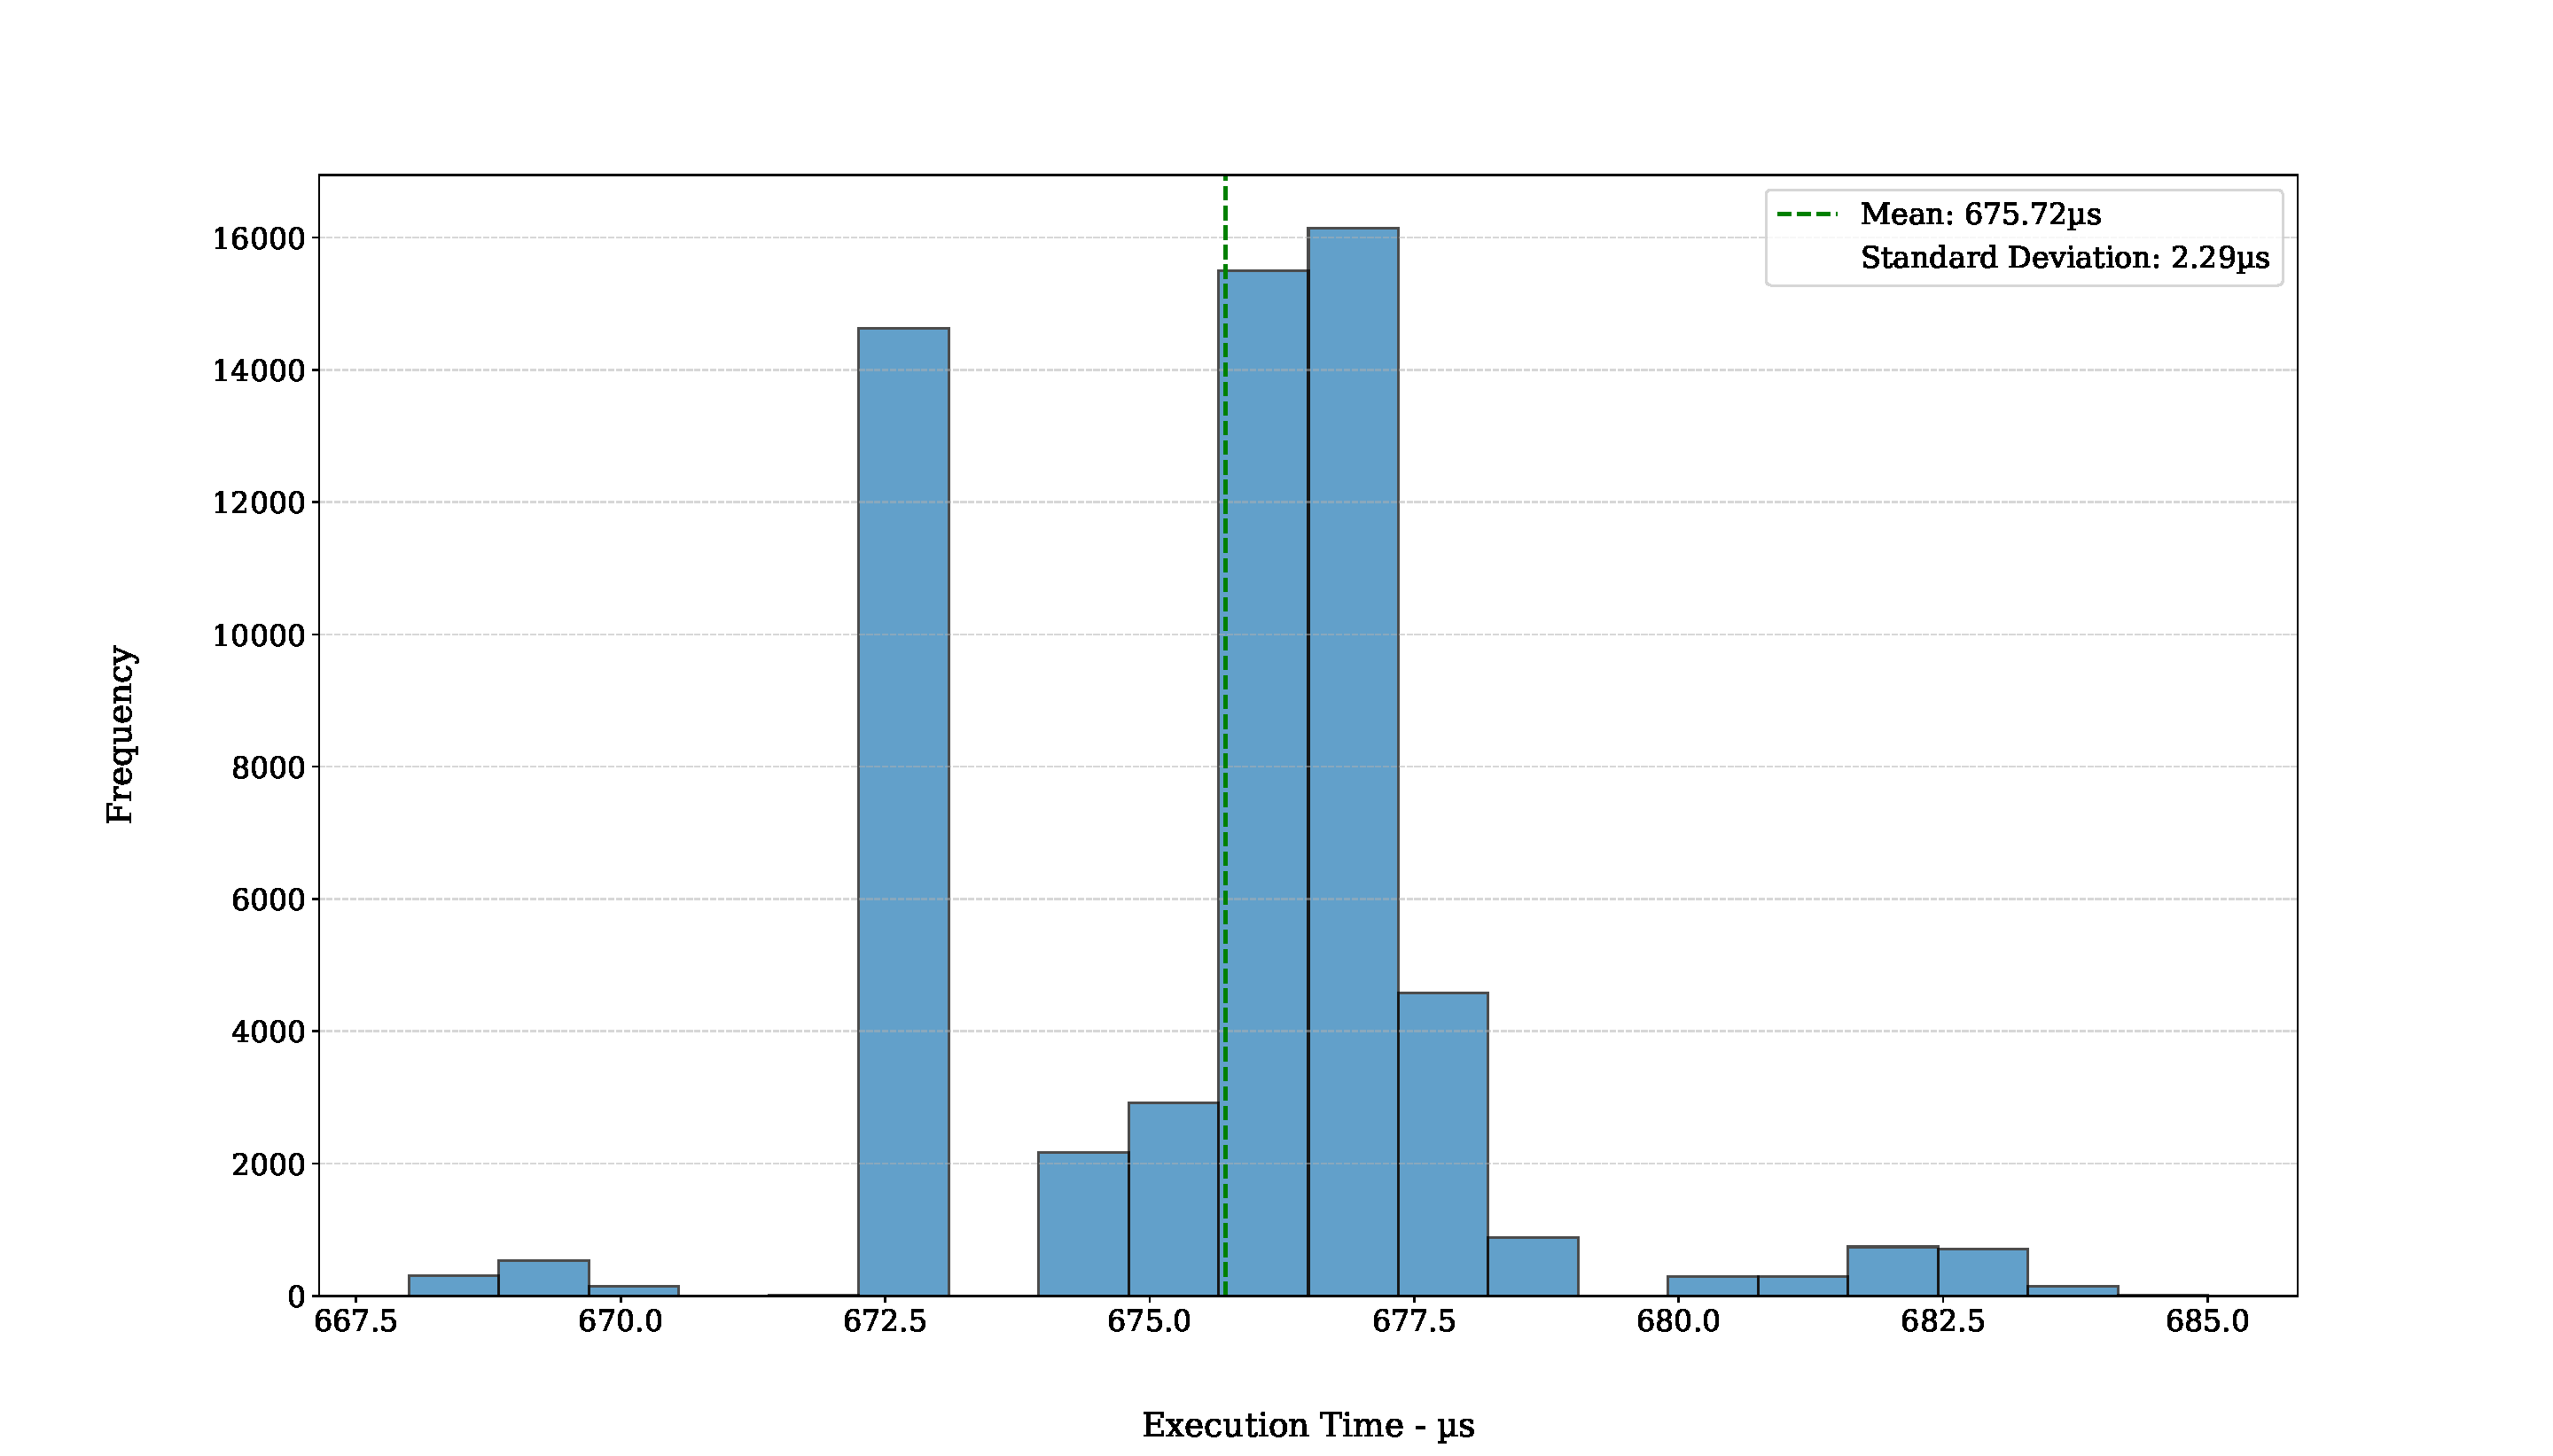
\includegraphics[width=0.95\textwidth]{images/16_with_linux_bandwidth.pdf}
	\caption{Tempos de Execução Das Iterações de Uma \gls{vm} Com Carga em CPU - Com Linux Invalidando Cache.}
    \label{fig:16_with_linux_bandwidth}
\end{figure}

\begin{figure}[ht]
    \centering
    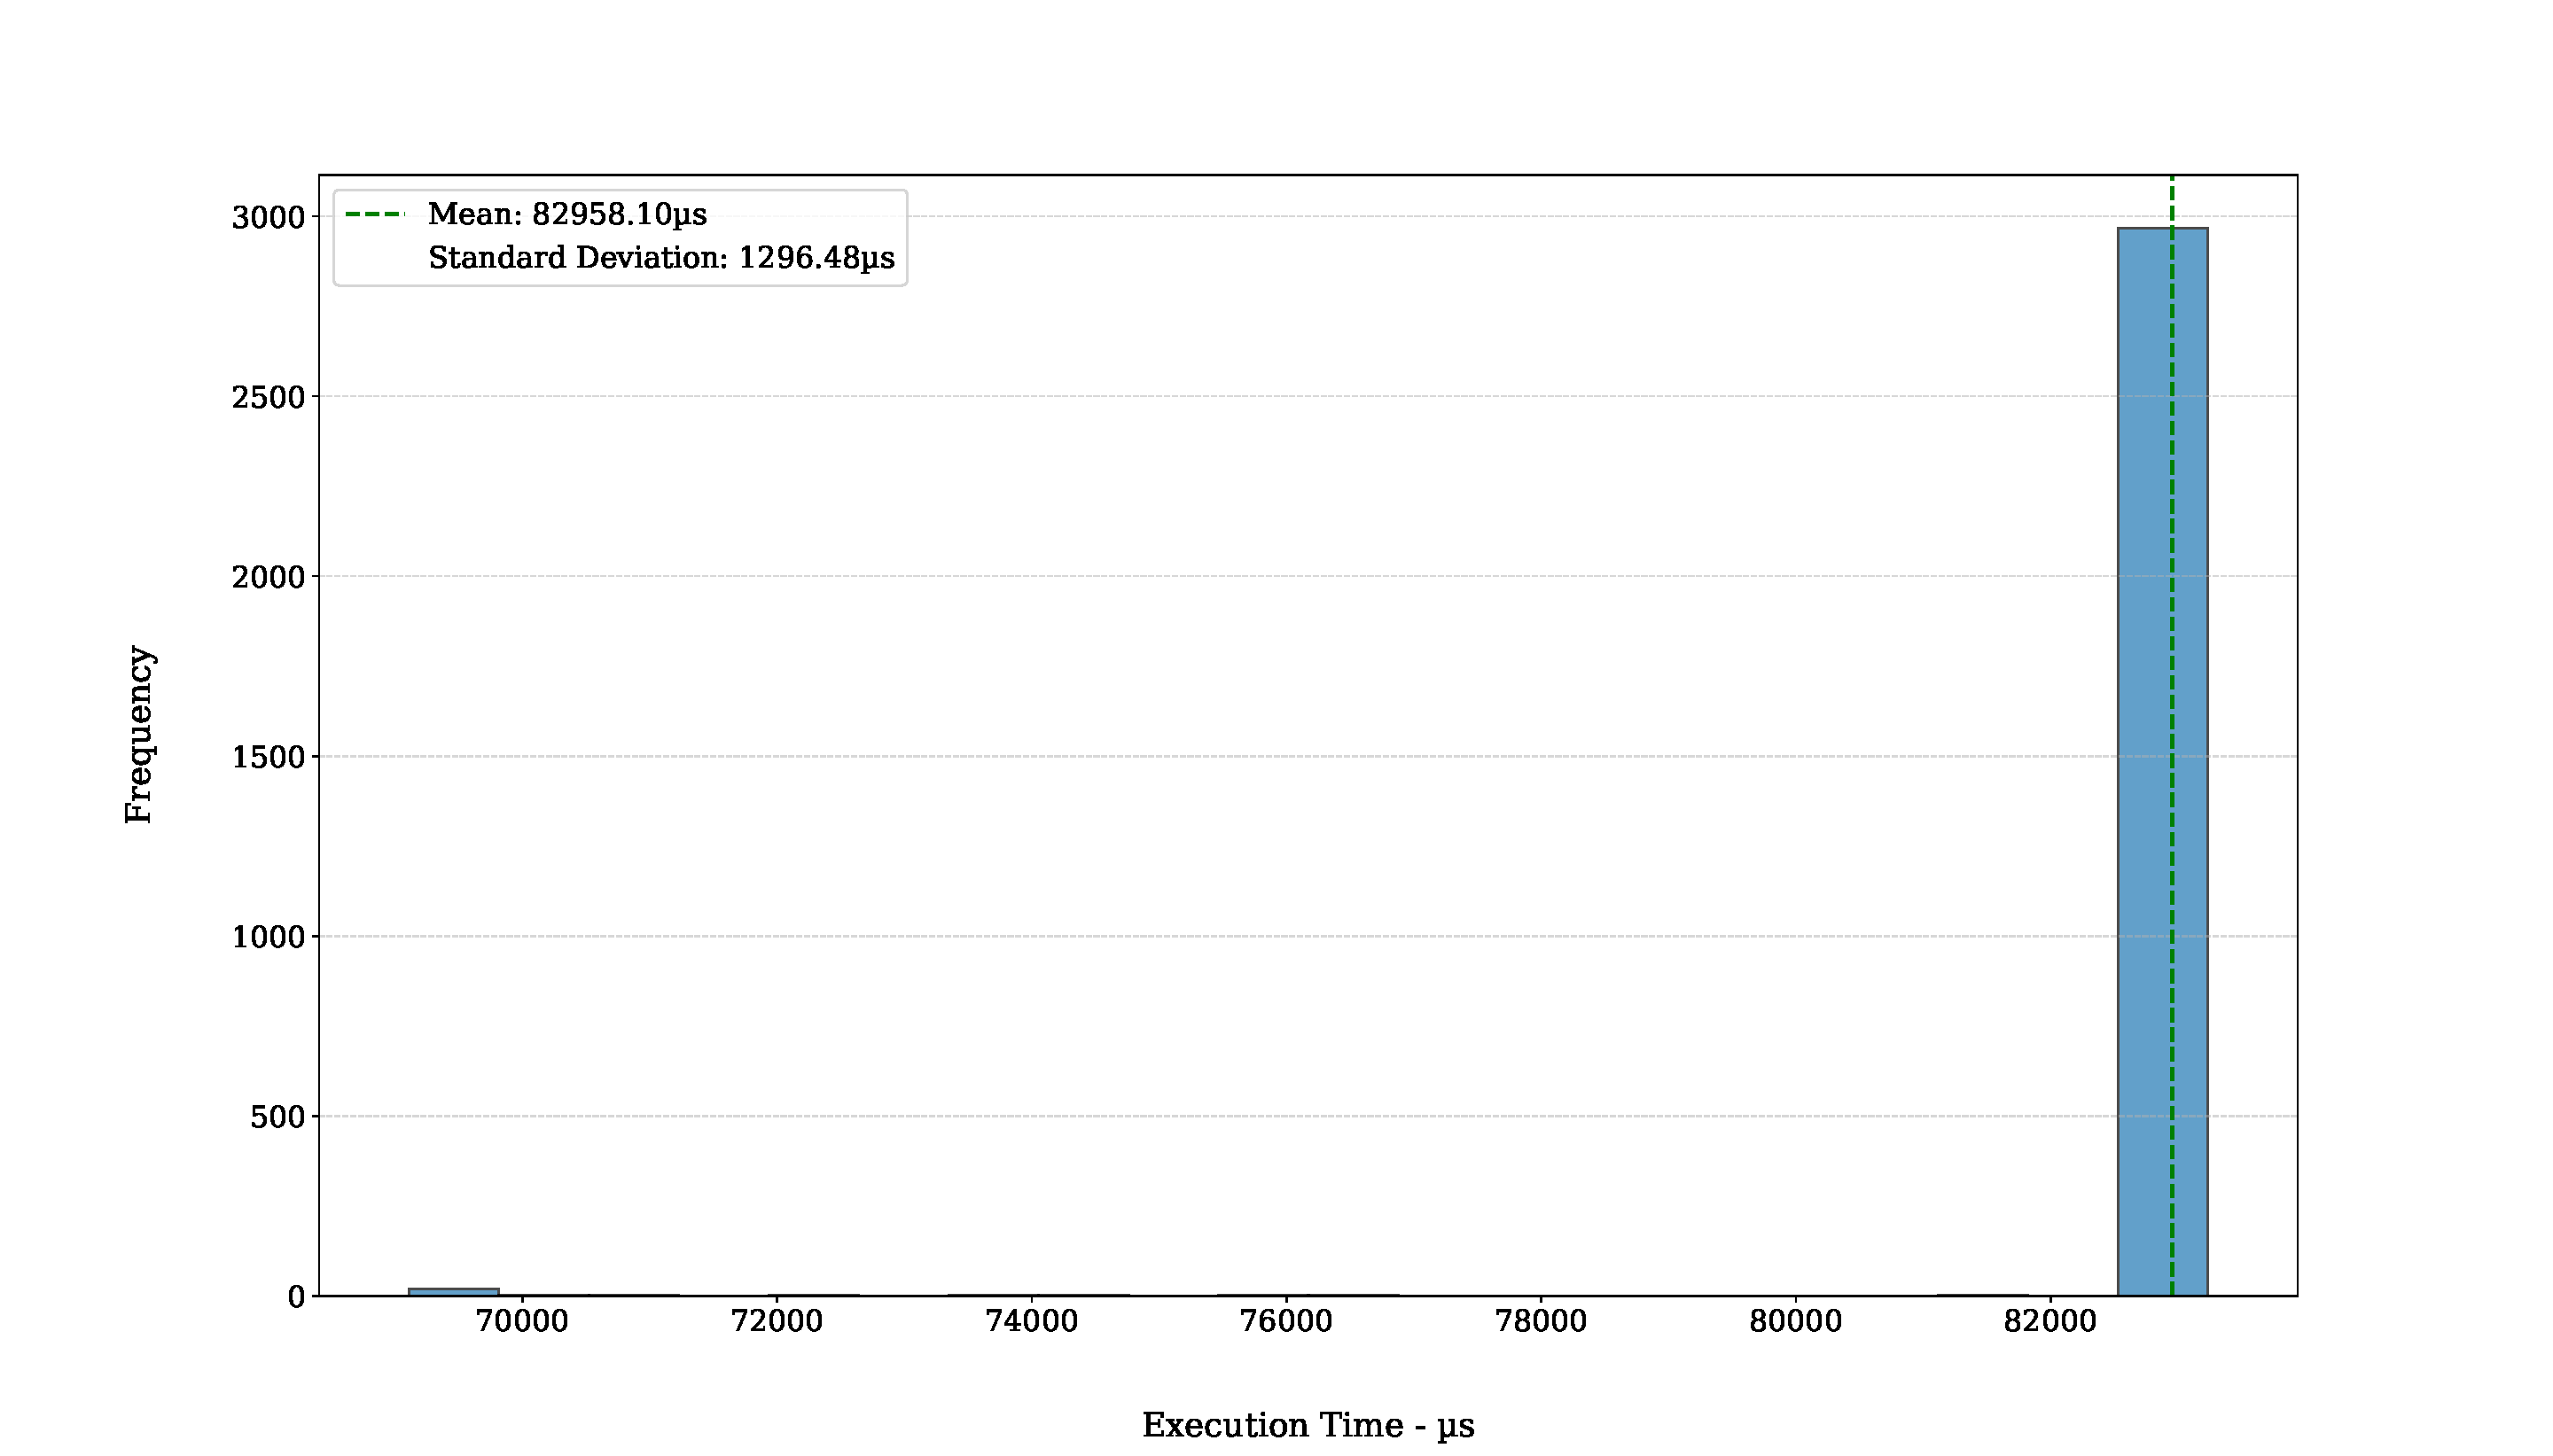
\includegraphics[width=0.95\textwidth]{images/23_with_linux_bandwidth.pdf}
	\caption{Tempos de Execução Das Iterações de Uma \gls{vm} Com Carga em Memória - Com Linux Invalidando Cache.}
    \label{fig:23_with_linux_bandwidth}
\end{figure}
